\documentclass[letter, 11pt]{article}
%% ================================
%% Packages =======================
\usepackage[utf8]{inputenc}      %%
\usepackage[T1]{fontenc}         %%
\usepackage{lmodern}             %%
\usepackage[spanish]{babel}      %%
\decimalpoint                    %%
\usepackage{fullpage}            %%
\usepackage{fancyhdr}            %%
\usepackage{graphicx}            %%
\usepackage{amsmath}             %%
\usepackage{color}               %%
\usepackage{mdframed}            %%
\usepackage[colorlinks]{hyperref}%%
%% ================================
%% ================================

%% ================================
%% Page size/borders config =======
\setlength{\oddsidemargin}{0in}  %%
\setlength{\evensidemargin}{0in} %%
\setlength{\marginparwidth}{0in} %%
\setlength{\marginparsep}{0in}   %%
\setlength{\voffset}{-0.5in}     %%
\setlength{\hoffset}{0in}        %%
\setlength{\topmargin}{0in}      %%
\setlength{\headheight}{54pt}    %%
\setlength{\headsep}{1em}        %%
\setlength{\textheight}{8.5in}   %%
\setlength{\footskip}{0.5in}     %%
%% ================================
%% ================================

%% =============================================================
%% Headers setup, environments, colors, etc.
%%
%% Header ------------------------------------------------------
\fancypagestyle{firstpage}
{
  \fancyhf{}
  \lhead{
\includegraphics[height=4.5em]{LogoDFI.jpg}}
  \rhead{FI3104-1 \semestre\\
         Métodos Numéricos para la Ciencia e Ingeniería\\
         Prof.: \profesor}
  \fancyfoot[C]{\thepage}
}

\pagestyle{plain}
\fancyhf{}
\fancyfoot[C]{\thepage}
%% -------------------------------------------------------------
%% Environments -------------------------------------------------
\newmdenv[
  linecolor=gray,
  fontcolor=gray,
  linewidth=0.2em,
  topline=false,
  bottomline=false,
  rightline=false,
  skipabove=\topsep
  skipbelow=\topsep,
]{ayuda}
%% -------------------------------------------------------------
%% Colors ------------------------------------------------------
\definecolor{gray}{rgb}{0.5, 0.5, 0.5}
%% -------------------------------------------------------------
%% Aliases ------------------------------------------------------
\newcommand{\scipy}{\texttt{scipy}}
%% -------------------------------------------------------------
%% =============================================================
%% =============================================================================
%% CONFIGURACION DEL DOCUMENTO =================================================
%% Llenar con la información pertinente al curso y la tarea
%%
\newcommand{\tareanro}{6}
\newcommand{\fechaentrega}{23/12/2020 23:59 hrs}
\newcommand{\semestre}{2020B}
\newcommand{\profesor}{Valentino González}
%% =============================================================================
%% =============================================================================


\begin{document}
\thispagestyle{firstpage}

\begin{center}
  {\uppercase{\LARGE \bf Tarea \tareanro}}\\
  Fecha de entrega: \fechaentrega
\end{center}


%% =============================================================================
%% ENUNCIADO ===================================================================

\vspace{1em}
\noindent{\large \bf Problema 1}\\
\noindent {\bf(Sin informe.)}

El archivo \texttt{GLB.Ts+dSST.csv} es un archivo de datos separado por comas.
Los datos provienen del \emph{Goddard Institute for Space Science} (GISS) y
contienen información sobre las anomalías de temperatura medidas en la tierra y
los océanos a lo largo de los años. Para ser precisos, la columna titulada
\texttt{J-D} indica la diferencia entre la temperatura base (elegida como la
temperatura promedio entre los años 1951 y 1980) y el promedio anual
(\emph{January-December}) para ese año, el cual se indica en la columna
titulada \texttt{Year}.

Asumiendo que no hacemos nada para alterar la tendencia mostrada por los datos,
estime para qué año la temperatura habrá cambiado en 2 grados celsius. Indique
a través de un comentario en su código qué forma paramétrica escogió y qué
algoritmo de minimización usó. Su código debe imprimir en pantalla un intervalo
de confianza para el año de la catástrofe más grande en la historia de la
humanidad
(\href{http://theconversation.com/why-is-climate-changes-2-degrees-celsius-of-warming-limit-so-important-82058}{artículo
random al respecto}), y producir un gráfico mostrando el mejor fit.

\begin{ayuda}
  \noindent Si le interesa obtener más información sobre los datos utilizados
  en esta pregunta, consulte la siguiente página:
  \href{https://data.giss.nasa.gov/gistemp/}{https://data.giss.nasa.gov/gistemp/}
\end{ayuda}


\vspace{1em}
\noindent{\large \bf Problema 2}\\
\noindent {\bf  (CON INFORME.)}

La técnica de la espectroscopía consiste en estudiar la radiación emitida por
una fuente como función de la longitud de onda. Las características de los
espectros observados nos permiten entender las propiedades físicas del ente
emisor de la radiación.

En la figura a continuación, se observa un segmento del espectro de una fuente
que muesta una leve pendiente y una línea de absorción. Las unidades son de
flujo por unidad de frecuencia $f_\nu [{\rm erg\ s^{-1} Hz^{-1} cm^{-2}}]$ vs.
longitud de onda en [Angstrom]. Su trabajo consiste en modelar simultáneamente
el contínuo con inclinación y la línea de absorción de la figura (los datos los
encontrará en el archivo \texttt{espectro.dat}).

Las líneas de absorción son en teoría casi infinitamente delgadas (hay un
ensanchamiento intrínseco dado por el principio de incertidumbre pero es muy
pequeño). Las observaciones, sin embargo, siempre muestran líneas mucho más
anchas. Dependiendo del mecanismo físico que produce el ensanchamiento, la
forma de la línea será distinta. Ud. deberá modelar la línea asumiendo el
mechanismo de ensanchamiento más típico, el cual produce líneas gaussianas.

El modelo completo será el de una línea recta para el contínuo (2 parámetros)
menos una función gaussiana con 3 parámetros: amplitud, centro y varianza. Es
decir, debe modelar 5 parámetros a la vez.

\begin{ayuda}
    \texttt{scipy.stats.norm} implementa la función Gaussiana si no quiere
    escribirla Ud. mismo. La forma de usarla es la siguiente: \texttt{g = A *
    scipy.stats.norm(loc=mu, scale=sigma).pdf(x)}; donde x es la longitud de
    onda donde evaluar la función.
\end{ayuda}

\begin{center}
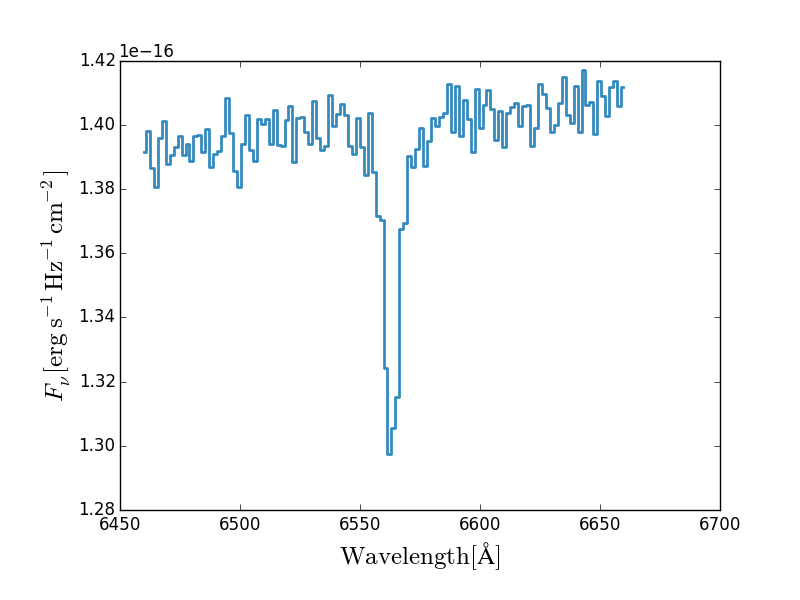
\includegraphics[width=0.6\textwidth]{spectrum.png}
\end{center}

Produzca un gráfico que muestre el espectro observado y el mejor fit obtenido.
Provea una tabla con los mejores parámetros, su error estándard y reporte el
valor de $\chi^2_{\rm reducido}$ en su mínimo.

Para buscar el mejor modelo recuerde que es importante dar un punto de partida
que sea cercano al mínimo para que los algoritmos converjan de manera efectiva.
Ud. debe idear un método para buscar ese punto de partida y explicitarlo en su
informe.



\vspace{2em}
\noindent\textbf{Instrucciones Importantes.}
\begin{itemize}

\item Para reducir la cantidad de trabajo necesaria para completar esta tarea,
  sólo debe escribir un informe para el Problema 2. De todos modos debe
  entregar el código escrito para ambos problemas.

 \item Repartición de puntaje:

   \subitem - 30\% Código y gráfico del Problema 1. Implementación y resolución
   del problema.
     
   \subitem - 30\% Código del Problema 2. Implementación y resolución del
   problema.

   \subitem - 30\% Informe Problema 2. Demuestra comprensión del problema y su
   solución, claridad del lenguaje, calidad de las figuras y/o tablas
   utilizadas. Para esta tarea el informe probablemente no require más de 3
   páginas pero esto es sólo una referencia.

   \subitem - 5\% Códigos aprueban a no \texttt{PEP8}.

   \subitem - 5\% Diseño del código: modularidad, uso efectivo de nombres de
   variables y funciones, docstrings, \underline{uso de git}, etc

\item Evaluaremos su uso correcto de \texttt{python}. Si define una función
  relativametne larga o con muchos parámetros, recuerde escribir el
  \emph{docstring} que describa los parámetros que recibe la función, el
  output, y el detalle de qué es lo que hace la función. Recuerde que
  generalmente es mejor usar varias funciones cortas (que hagan una sola cosa
  bien) que una muy larga (que lo haga todo).  Utilice nombres explicativos
  tanto para las funciones como para las variables de su código. El mejor
  nombre es aquel que permite entender qué hace la función sin tener que leer
  su implementación ni su \emph{docstring}.

\item Su código debe aprobar la guía sintáctica de estilo
  (\href{https://www.python.org/dev/peps/pep-0008/}{\texttt{PEP8}}). En
  \href{http://pep8online.com}{esta página} puede chequear si su código aprueba
  \texttt{PEP8}.

\item Utilice \texttt{git} durante el desarrollo de la tarea para mantener un
  historial de los cambios realizados. La siguiente
  \href{https://education.github.com/git-cheat-sheet-education.pdf}{cheat
    sheet} le puede ser útil. {\bf Revisaremos el uso apropiado de la
  herramienta y asignaremos una fracción del puntaje a este ítem.} Realice
  cambios pequeños y guarde su progreso (a través de \emph{commits})
  regularmente. No guarde código que no corre o compila (si lo hace por algún
  motivo deje un mensaje claro que lo indique). Escriba mensajes claros que
  permitan hacerse una idea de lo que se agregó y/o cambió de un
  \texttt{commit} al siguiente.

\item Al hacer el informe usted debe decidir qué es interesante y agregar las
  figuras correspondientes. No olvide anotar los ejes, las unidades e incluir
  una \emph{caption} o título que describa el contenido de cada figura.

\item La tarea se entrega subiendo su trabajo a github. Trabaje en el código y
  en el informe, haga \textit{commits} regulares y cuando haya terminado
  asegúrese de hacer un último \texttt{commit} y luego un \texttt{push} para
  subir todo su trabajo a github. \textbf{REVISE SU REPOSITORIO PARA ASEGURARSE
  QUE SUBIÓ LA TAREA. SI UD. NO PUEDE VER SU INFORME EN GITHUB.COM, TAMPOCO
PODREMOS NOSOTROS.}

\item El informe debe ser entregado en formato \texttt{pdf}, este debe ser
  claro sin información de más ni de menos. \textbf{Esto es muy importante, no
  escriba de más, esto no mejorará su nota sino que al contrario}. La presente
  tarea probablemente no requiere informes de más de 3 páginas. Asegúrese de
  utilizar figuras efectivas y tablas para resumir sus resultados.

\item \textbf{REVISE SU ORTOGRAFÍA.}


\end{itemize}
%% FIN ENUNCIADO ===============================================================
%% =============================================================================

\end{document}
